\chapter{Evaluation}
\label{cha:evaluation}
This section provides an overview of a set of metrics established to compare the developed campus app to already established routing solutions for mobile devices (Google Maps and Apple Maps), highlight the benefits of the campus app over the manual campus map provided by TU Berlin and measure the improvement of usability when compared to TU Berlin's online web resources. Furthermore, all steps regarding implementation, data acquisition and measurement as well as the resulting consequences for the respective metric are presented.

\section{Campus map verfication} \label{sec:campus_map_verification}
The digital campus map of TU Berlin forms the app's most important element. It is therefore essential to evaluate and compare its implementation to other digital maps. This section presents an overview of different metrics that can be evaluated quantitatively for map verification and compares the actual measurements to the geolocation services of Android and IOS.

To verify the campus map, an important emphasis must be laid on the correctness and quality of the underlying geodata. To achieve this, two different benchmarks, one for measuring the geographical resolution of a map and one for measuring its geocoding capabilities, are introduced in the following sections.

%the map resolution of campus Charlottenburg, which indicates the level of detail on the map, as well as the geocoding capabilities of the system, %mainly the mapping of university-specific identifiers and names to their respective campus entities, are compared.

%Einmal die Abstände bei zufälligen Koordinaten und zwischen Gebäude-Koordinaten und den Eingängen messen
\subsection{Comparison of map resolution}
The geographical resolution of a map describes the level of detail that the underlying geodata has. A more detailed set of geodata can result in better map visualization for the user interface (improving usability as well as localization capabilities) and a more complex underlying navigation graph that can calculate individual routes more precisely.

To measure a comparable indicator for the geographical resolution of a particular map, the underlying geocoding API of the respective mobile app provider is used. This API provides the possibility to query the system's most fitting geodata points for a particular geographical input (pair of latitude and longitude).

It can be assumed that the distances of the candidate points returned by a geocoding API to the original point can be seen as a metric that indicates the geodata coverage of the specified region, with low distances suggesting that the system contains an adequate representation of the area around the geographic campus point. The following list describes the set of steps that are performed to measure this map resolution metric for the whole campus:

\newpage

\begin{enumerate}
    \item A random set of $N$ geographical points $P = \{p_{0}, p_{1}, p_{2}, \ldots\}$, each lying on campus Charlottenburg, is generated
    \item The set of the system's most fitting candidate points $C_{i} = \{c_{i_{0}}, c_{i_{1}}, c_{i_{2}}, \ldots\}$ is queried for each random point $p_{i}$ from the respective geocoding API
    \item The distances $D_{i} = \{dist(p_{i}, c_{i_{0}}), dist(p_{i}, c_{i_{1}}), dist(p_{i}, c_{i_{2}}), \ldots\}$ are calculated
    \item The minimal distance $d_{i} = \min(D_{i})$ for each point $p_{i}$ is retrieved and the average of all minimal distances $\frac{d_{0} + d_{1} + d_{2} + \cdots + d_{N}}{N}$ for a specific geocoding provider is calculated
    \item These averaged values are compared between geocoding engines and provide an indicator for the geographical node coverage of each system's campus representation
\end{enumerate}

\vspace{2mm}

For practical implementation, the campus is split into 3 bounding boxes \ref{table:campus_regions}. A total of 250 random geographic points are generated for each bounding box and the average closest point distances are calculated for each campus region and each geocoding provider API (campus app, Android and IOS). The following figure presents the results:

\begin{figure}[H]
	\centering
	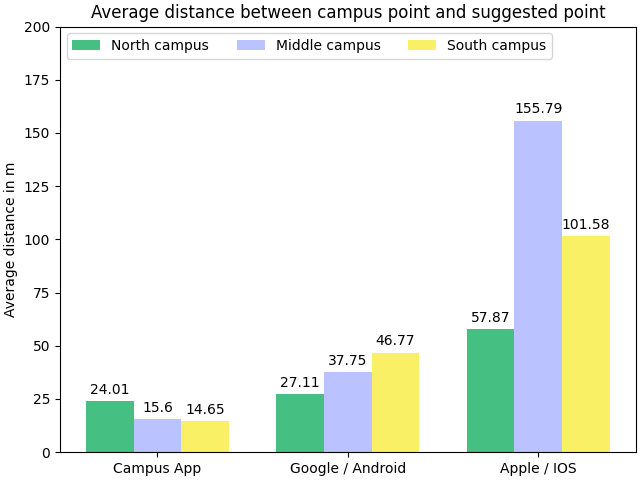
\includegraphics[width=0.75\textwidth]{images/average_campus_point_distance.png}\\
	\caption{Average distance between campus point and suggested point}
\end{figure}

The figure shows that the campus app outperforms the geocoding capabilities of the Android and IOS operating system geocoding services on randomly sampled point datasets for every region of campus Charlottenburg by factors 1 to 3 for Google Maps and 2 to 10 for Apple Maps.

The values for the entire campus are 18,08 m for the campus app, 37,21 m (approx. factor 2) for Google Maps and 105,08 m (approx. factor 5) for Apple Maps. When extrapolated for the entirety of all geographical points on the campus, it can be concluded that the overall resolution of campus Charlottenburg differs by presented factors between those geocoding APIs.

\newpage

To provide a more differentiated evaluation of the campus coverage, a set of heatmaps is created, each displaying the map of campus Charlottenburg with the geodata coverage of the respective geocoding API.

\begin{figure}[H]
	\centering
	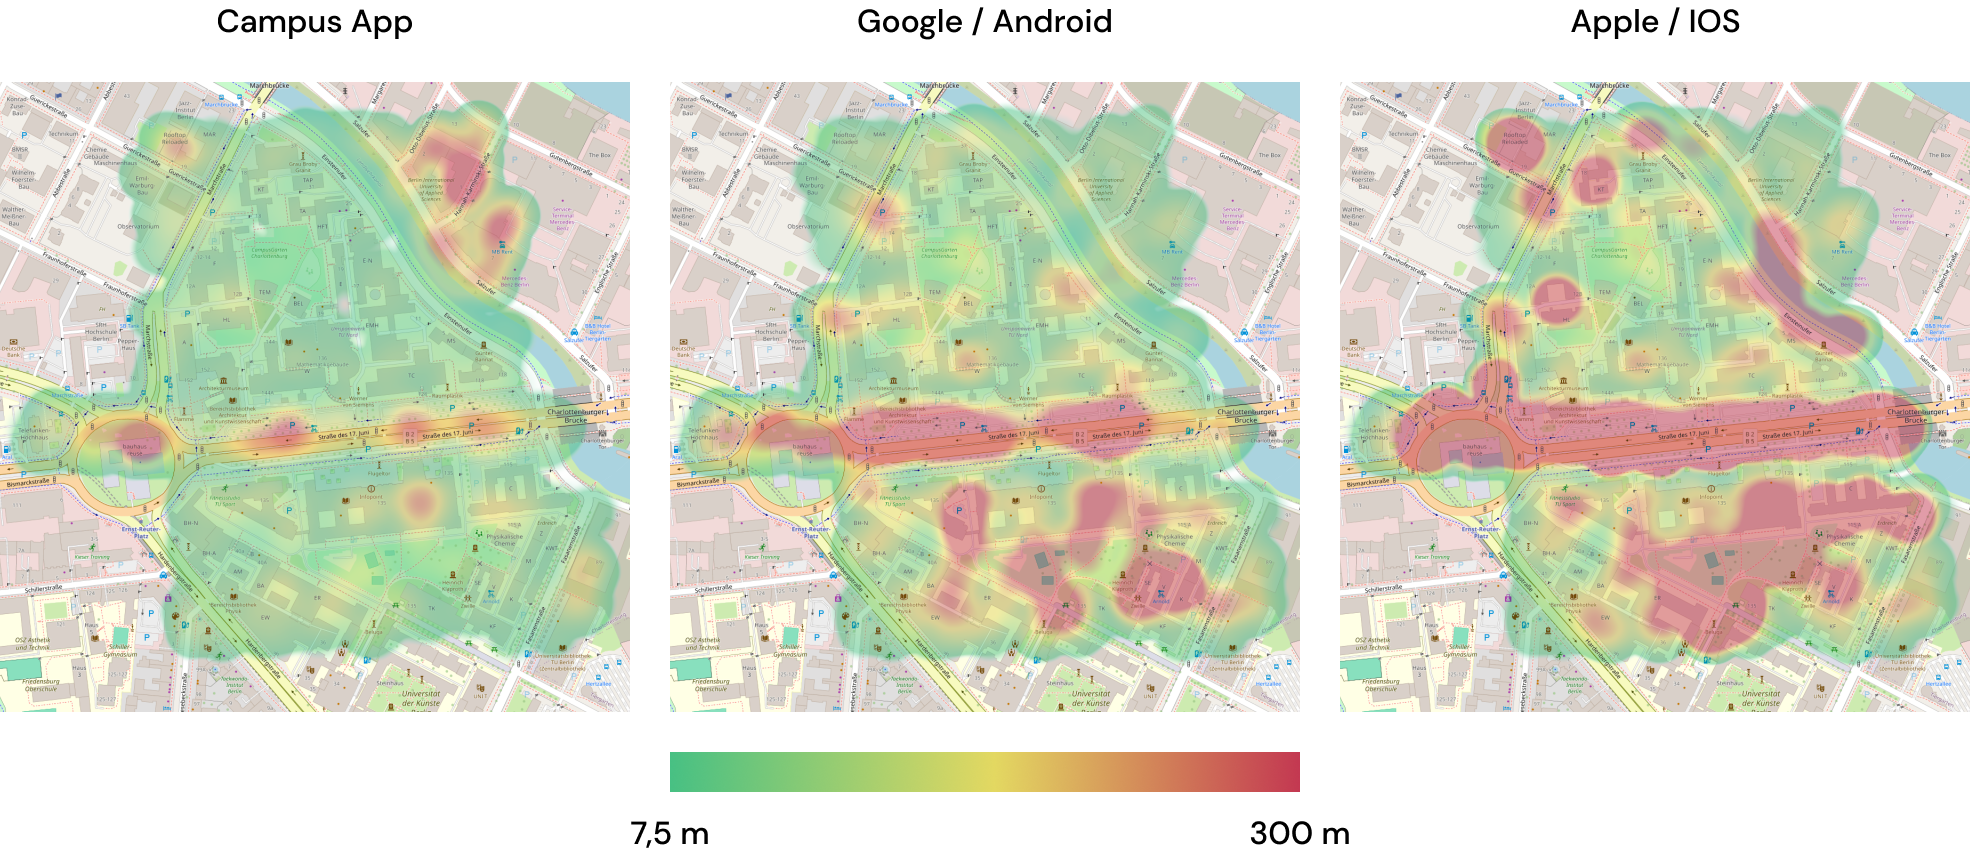
\includegraphics[width=1.0\textwidth]{images/heatmaps.png}\\
	\caption{Heatmaps for campus map coverage by average point distance}
\end{figure}

One important factor that can be drawn from both data representations is the fact that the north side of campus Charlottenburg has a better geodata coverage than the south side and the middle section throughout all different providers. The heatmaps also present the fact that the campus app has the best average campus resolution and that its resolution weaknesses can (since no important entity or pathway is located in these areas) be seen as negligible for the proper functionality of the system.

Generally can be said that the Android geolocation services are more precise than the IOS counterparts in the scope of campus Charlottenburg. Both systems nevertheless struggle when points are queried for the south side of campus Charlottenburg as well as for Straße des 17. Juli. The latter weakness mostly arises from the fact that every geolocation in the campus-splitting section of Straße des 17. Juli gets mapped onto the TU main building.

\subsection{Comparison of geocoding capabilities for campus-specific names and identifiers}
One important factor for the usability of a geocoding system is the resolution of human-readable entity names and identifiers into their respective geographic coordinates. Regarding the focus on TU Berlin's campus in Charlottenburg, a system should be able to correctly identify the building's abbreviations (e.g., TEL, MAR, H, \ldots) as well as their official names (e.g., TU-Hochhaus, Marchstraße-Gebäude, Hauptgebäude, \ldots). This section provides a benchmark to measure this ability across the geocoding APIs of the campus app, Google / Android and Apple / IOS.

To perform such a benchmark, a dataset is established, containing the entirety of the campus-specific identifiers (abbreviations) and official names of TU Berlin's entities. In exceptional cases, additional commonly used building names (e.g., "Telefunken Hochhaus" instead of "TU-Hochhaus") are also added to the dataset. This dataset is then fed into the respective geocoding APIs and the sets of possible candidate points for each query are retrieved. If at least one of the resulting candidate points is located close enough to the respective center coordinates of the inputted entity (in the test case less than 100 meters away), the human-readable input is counted as recognized by the system. To compensate for the fact that the Android and IOS geocoding APIs are not focussed on TU Berlin's campus entities, the suffix "TU Berlin" is added to each query, mimicking a common user behavior when searching for campus entities in both respective mobile apps. Furthermore, the geocoding of the actual address for each building is also analyzed for reference. The following figure presents the results.

\begin{figure}[H]
	\centering
	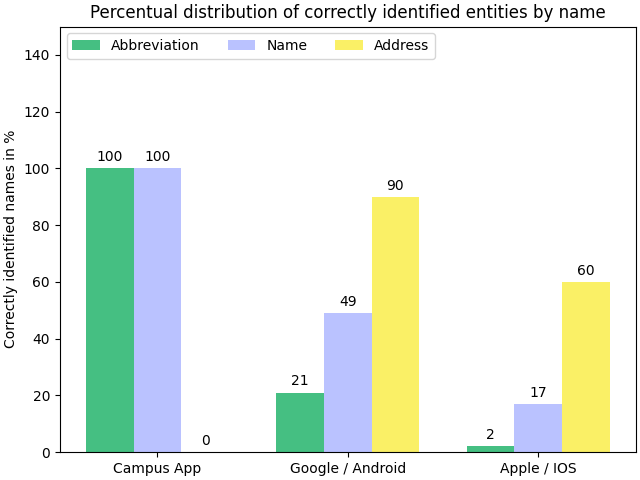
\includegraphics[width=0.75\textwidth]{images/results_geocoding_identifiers.png}\\
	\caption{Average distance between campus point and suggested point}
\end{figure}

The campus app surpasses the geocoding capabilities of Google and Apple in terms of knowledge of entity abbreviations and names. Furthermore, Google outperforms Apple throughout all categories, but both systems struggle to detect an adequate amount of abbreviations. The name metrics are in the midfield, while the systems tend to perform better when resolving direct building addresses.

\section{Navigation system verification} \label{sec:navigation_system_verification}
One important criterion for navigation system verification lies in the quality of the routes suggested by it. A route is thereby defined as the suggested path between a specified start and destination point, which, in the case of this thesis, are both part of TU Berlin's main campus in Charlottenburg. To analyze named quality for a specific route, the estimated time it takes to walk as well as its length are both measured. Lower walking times, as well as shorter route lengths, are thereby both regarded as preferable.

To perform a comparison between different navigation systems, a set of predefined start and destination points is established. The route calculation process of each navigation system is then applied to the defined reference points and the route metrics of the suggested routes are collected respectively. The navigation systems can be then compared for a specific pair of start and destination points as well as for the average metrics of the whole dataset. 

The pool of reference points for this comparison is chosen from the underlying building data of TU Berlin. Each center point of a building is added to the set and can be used as a starting and destination point for route calculation. The navigation systems therefore calculate all possible routes between TU Berlin's buildings. This comes with two advantages: On the one hand, the chosen pool of possible routes is large enough to be quantitatively meaningful. On the other hand, the navigation between different buildings portrays a common task for the target audience of the campus app and therefore mimics the expected user behavior. The chosen pool of reference points is furthermore representative of the geographical structure of campus Charlottenburg.

The following table presents the average results for the entire reference point dataset measured respectively on the campus app, Google Maps and Apple Maps.

\begin{table}[H]
	\small
	\centering
	\begin{tabular}{|l|l|l|}
		\hline
		\textbf{Navigation system}      & \textbf{Average walking time}       & \textbf{Average route length}  \\
		\hline
        Campus App             & 6 min 44 s	              	& approx. 510 m         \\
		\hline
        Google Maps            & 9 min 30 s              	& approx. 690 m         \\
		\hline
		Apple Maps             & 9 min 38 s              	& approx. 670 m         \\
		\hline
	\end{tabular}
	\caption{Comparison of walking time and route length}
\end{table}

The measured key figures suggest average time savings of 30\% (Google Maps) and 30\% (Apple Maps) as well as average distance savings of 23\% (Google Maps) and 20\% (Apple Maps) when the route recommended by the campus app is chosen over its counterparts. To further analyze the underlying factors for this speedup, the percentual route metrics are split according to the underlying route length suggested by the campus app:

\begin{figure}[H]
	\centering
	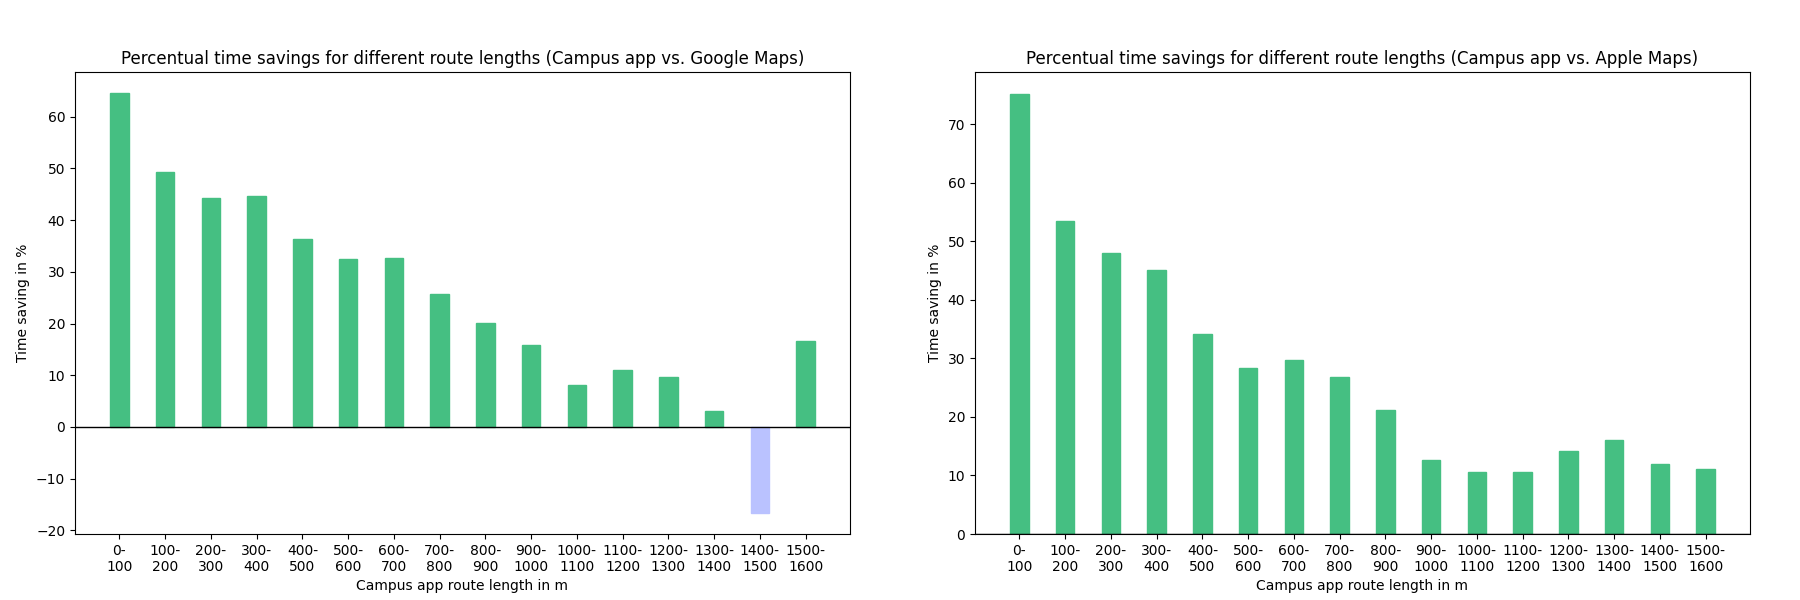
\includegraphics[width=1.0\textwidth]{images/time_differences.png}\\
	\caption{Average percentual time savings for different route lengths}
\end{figure}

\begin{figure}[H]
	\centering
	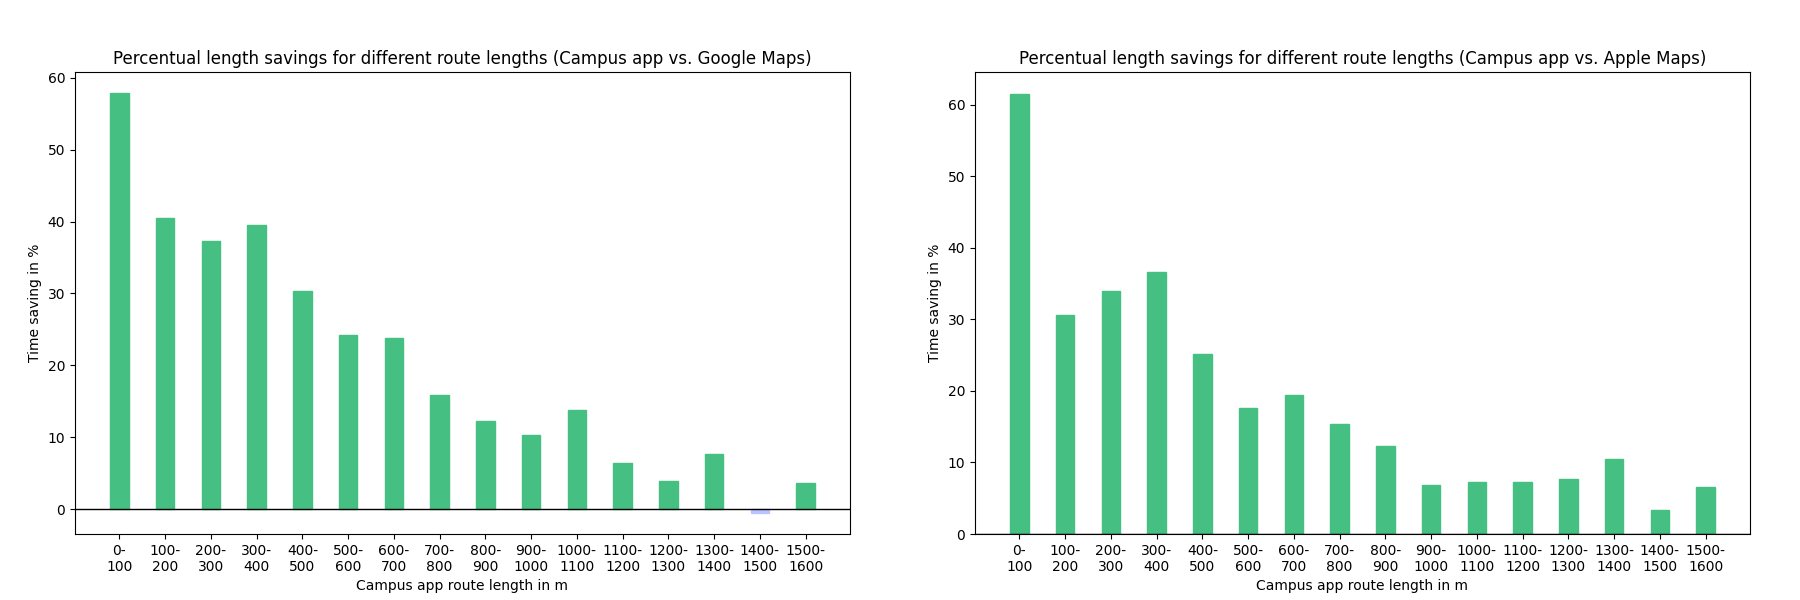
\includegraphics[width=1.0\textwidth]{images/length_differences.png}\\
	\caption{Average percentual distance savings for different route lengths}
\end{figure}

One main evaluation point that can be derived from the plots is the fact that through all route length categories (except for the distance interval of 1.4 km to 1.5 km in the Google Maps comparison), the suggested routes from the campus app always result in faster and shorter paths. This speedup is especially high for shorter routes (< 700 m) and declines with increasing route length. The overall biggest speedup is achieved in the category for routes under 100 meters. In this section, start and destination points often lay in different but connected buildings. The routing for this circumstance can be solved very efficiently by the campus app as an indoor route between both buildings can be proposed.

% \section{Information layer verification}
